\documentclass{article}
\usepackage[utf8]{inputenc}
\usepackage[spanish,es-tabla,es-nodecimaldot]{babel}
\usepackage{enumitem}
\usepackage{graphicx}
\graphicspath{ {reports/figures/} }
\usepackage{textcomp}
\usepackage{color}
\usepackage{upquote,listings}
%\usepackage{lscape}
\usepackage{pdflscape}


\definecolor{codegreen}{rgb}{0,0.6,0}
\definecolor{codegray}{rgb}{0.5,0.5,0.5}
\definecolor{codepurple}{RGB}{219, 48, 122}
\definecolor{backcolour}{RGB}{242, 242, 242}
\definecolor{bookColor}{cmyk}{0,0,0,0.90}  
\color{bookColor}

\lstset{upquote=true}

\lstdefinestyle{mystyle}{
    backgroundcolor=\color{backcolour},   
    commentstyle=\color{codegreen},
    keywordstyle=\color{codepurple},
    numberstyle=\numberstyle,
    stringstyle=\color{codepurple},
    basicstyle=\footnotesize\ttfamily,
    breakatwhitespace=false,
    breaklines=true,
    captionpos=b,
    keepspaces=true,
    numbers=left,
    numbersep=10pt,
    showspaces=false,
    showstringspaces=false,
    showtabs=false,
}
\lstset{style=mystyle}

\newcommand\numberstyle[1]{%
    \footnotesize
    \color{codegray}%
    \ttfamily
    \ifnum#1<10 0\fi#1 |%
}


\title{Normalización de base de datos del Directorio Estadístico de Unidades Económicas (DENUE).}
\author{
    Ana Maritza Bello Yañez
}

\date{\today}

\begin{document}
\maketitle


\begin{abstract}
    En esta práctica se crearon 7 catálogos a partir de la base de datos del
    DENUE. La finalidad de crear estos catálogos es disminuir el espacio ocupado
    por la base de datos original. Finalmente, se logró disminuir el espacio de
    236 a 184 MB, con lo que logramos el onjetivo de la práctica.
    Como trabajo a futuro se recomienda realizar una normalización formal de la
    base de datos y llevarla en la medida de lo posible a una forma normal que
    permita una mejor manipulación de los datos y que ayude a disminuir su
    tamaño aún más.

    \subsection*{Objetivos}
    \begin{enumerate}
        \item Crear catálogos a partir de atributos que no tengan dependencia a
        otros atributos.
        \item Sustituir las llaves primarias de los catálogos creados en la base
        de datos original, de tal manera que las tablas estén relacionadas por
        llave primaria y foránea.
        \item Verificar que el espacio ocupado en disco por la base de datos
        disminuyó con la creación de catálogos.
    \end{enumerate}
\end{abstract}

\section{Introducción}

\subsection*{Normalización de bases de datos}

La normalización de una base de datos consiste en re-diseñarla en estructuras
más pequeñas. Esto se hace mediante la transformación de las vistas de usuario
complejas y de la base de datos a un juego de tablas de datos más pequeñas y
estables (catálogos).

Cuando una base de datos crece, al no tener un buen diseño, se crean varios
problemas; entre ellos la redundancia de datos, que es cuando repetimos la misma
información en muchos registros. Esta redundancia en los datos se traduce en
espacio en disco y con esto se crea también un problema de mantenimiento, ya que
si queremos actualizar un dato, es posible que tengamos que hacerlo en más de un
lugar, con lo que crece la posibilidad de cometer errores.

La finalidad de la normalización es mejorar el desempeño de la base de datos, es
decir, mejorar el diseño y eliminar datos que sean redundantes. Así, cuando
tengamos que actualizar un dato en una base de datos normalizada, solo lo
tendremos que cambiar en una tabla y evitaremos errores a la hora de
actualizarlo.

Cuando normalizamos una base de datos reducimos su espacio en disco ya que se
crean tablas más pequeñas sin datos repetidos. Las tablas generadas (catálogos)
estarán relacionadas entre sí a partir de una llave primaria o
\textit{primary\_key}, que será una columna que llevará la palabra
\textit{id} de identificador en el nombre. 

Los datos de la llave primaria generalmente son del tipo \textit{integer} ya que
los datos de este tipo ocupan un espacio de almacenamiento de 4 bytes, mientras
que un dato tipo \textit{string} de 15 caractéres usará hasta 19 bytes.

\subsection*{Datos del DENUE}

Para realizar esta práctica utilizamos los datos del DENUE 2022. Estos datos
contienen la información de 5,528,698 negocios en el país e incorpora las
actualizaciones de establecimientos, en especial, a partir del Estudio sobre la
Demografía de los Negocios 2021.

Los datos que publica el directorio sobre las unidades económicas son los
siguientes:

\begin{enumerate}
    \item Identificación
    \begin{itemize}
        \item Nombre de la unidad económica
        \item Denominación o razón social (personas morales)
        \item Estrato de personal ocupado
        \item Código y título o nombre de la clase de actividad económica
        \item Tipo de la unidad económica
    \end{itemize}

    \item Ubicación
    \begin{itemize}
        \item Domicilio postal o geográfico
        \item Tipo y nombre de vialidad
        \item Número exterior
        \item Edificio, piso o nivel
        \item Número interior
        \item Tipo y nombre del asentamiento humano
        \item Corredor industrial, centro comercial o mercado público
        \item Número de local
        \item Código Postal
        \item Área geoestadística Estatal (AGEE)
        \item Área geoestadística Municipal (AGEM)
        \item Localidad geoestadística
        \item Manzana
        \item Coordenadas de Latitud
        \item Coordenadas de Longitud
    \end{itemize}

    \item Contacto
    \begin{itemize}
        \item Número de teléfono
        \item Correo electrónico
        \item Sitio en internet
    \end{itemize}
    \item Fecha de incorporación al DENUE
\end{enumerate}

\section{Desarrollo}
Como primer paso renombramos las columnas de tal manera que los nombres quedaran
bien especificados y evitar ambigüedades. Ya que estamos trabajando solo con
datos de la ciudad de México, también se eliminaron las columnas de
\texttt{clave\_entidad} y \texttt{entidad}, ya que estas contenían los datos
\texttt{09} y \texttt{Ciudad de México} respectivamente, repetidos en todos los
registros.

\lstinputlisting[language=SQL,   
framesep=10pt,
framextopmargin=10pt]
{../src/rename_columns.sql}

\subsection{Creación de catálogos}
Para reducir el espacio ocupado en disco de la base de datos del DENUE, creamos
6 catálogos de datos. Se escogieron atributos que fueran independientes de
otros, los catálogos creados fueron los siguientes:

\begin{enumerate}
    \item Catálogo de municipios.
    Los municipios o alcaldías de la Ciudad de México son 16 y ya que son un
    atributo independiente de los datos del DENUE (no cambia), optamos por hacer
    un catálogo de este.
    El código utilizado para generar este catálogo, es el siguiente:
    \lstinputlisting[language=SQL,   
        framesep=10pt,
        framextopmargin=10pt]
        {../src/municipios.sql}

    \item Catálogo de actividades económicas.
    Los tipos de actividades económicas ya están definidas por el DENUE, así que
    también es conveniente hacer un catálogo de estas.
    El código utilizado para generar este catálogo, es el siguiente:

    \lstinputlisting[language=SQL,   
    framesep=10pt,
    framextopmargin=10pt]
    {../src/actividades.sql}

    \item Catálogo de vialidades.
    Los tipos de vialidades que existen son 24. La conveniencia de crear un
    catálogo de estas es que tenemos 4 campos en los cuales podemos sustituir el
    valor por la llave foránea de este catálogo.
    El código utilizado para generar este catálogo, es el siguiente:

    \lstinputlisting[language=SQL,   
    framesep=10pt,
    framextopmargin=10pt]
    {../src/vialidades.sql}

    \item Catálogo de tipos de asentamientos.
    Los tipos de asentamiento humano ya están definidos, por lo que no cambiarán
    y es independiente de otro atributo. Los tipos de asentamientos son 43.
    El código utilizado para generar este catálogo, es el siguiente:

    \lstinputlisting[language=SQL,   
    framesep=10pt,
    framextopmargin=10pt]
    {../src/asentamientos.sql}

    \item Catálogo de centros comerciales.
    Se refiere al tipo de plaza, centro comercial, etc. donde se encuentra la
    unidad económica.
    El código utilizado para generar este catálogo, es el siguiente:

    \lstinputlisting[language=SQL,   
    framesep=10pt,
    framextopmargin=10pt]
    {../src/centros_comerciales.sql}

    \item Catálogo de Códigos Postales.

    El código utilizado para generar este catálogo, es el siguiente:

    \lstinputlisting[language=SQL,   
    framesep=10pt,
    framextopmargin=10pt]
    {../src/codigos_postales.sql}

    \item Catálogo de contactos de establecimientos.
    Este catálogo se creo con la finalidad de crear una tabla que contenga los
    datos de contacto del negocio, estos son:

    \begin{itemize}
        \item Teléfono
        \item Correo electrónico
        \item Página web
    \end{itemize}

    Dado que son atributos cuyo valor puede ser nulo o no, el hecho de ponerlos
    en una tabla aparte nos permite eliminar de la base de datos principal
    aquellos registros donde los tres campos están vacíos.

    El código utilizado para generar este catálogo, es el siguiente:

    \lstinputlisting[language=SQL,   
    framesep=10pt,
    framextopmargin=10pt]
    {../src/datos_de_contacto.sql}

\end{enumerate}

\subsection{Reemplazo de columnas por llave foránea}

Una vez creados los catálogos, sustituimos el \texttt{id} o llave primaria de
los catálogos en la base de datos original. El \texttt{id} de otra tabla llamado
en la base de datos principal se llama \textit{llave foránea}.

Después de sustituir las columnas originales por la llave foránea, ya tenemos
una nueva base de datos que está relacionada a las otras tablas a partir de
estas llaves.

El código a continuación es el utilizado para realizar esta sustitución.

\lstinputlisting[language=SQL,   
framesep=10pt,
framextopmargin=10pt]
{../src/actualiza_bd.sql}

\subsection{Uso del comando \texttt{vacuum full}}
Finalmente se utilizó el comando \texttt{vacuum full} ya que este reclama el
espacio ocupado por tuplas muertas. En PostgreSQL las tuplas que se eliminan o
que quedan obsoletas por un \texttt{update} no se remueven al instante de la
tabla, sino que quedan presentes hasta que se hace el \texttt{VACUUM}. Aunque
los gestores de bases de datos (en este caso el utilizado fue \textit{DBeaver})
realizan este vaciado de manera periódica, se recomienta realizarlo si es
necesario.


\section{Resultados y discusión}

La siguiente tabla muestra el tamaño de cada uno de los catálogos creados a
partir de la base de datos original. También podemos observar como baja el
tamaño de la base de datos original conforme actualizamos la llave foránea de
cada uno de los catálogos.

\begin{table}[h!]
    \centering
\begin{tabular}{c|c|c}
    Catálogo sustituido & Tamaño del catálogo & Tamaño de la base de datos\\
    \hline
    Base de datos original & No aplica & 236 MB \\
    Municipios & 24 KB & 222 MB \\
    Actividades & 152 KB & 195 MB \\
    Vialidades & 24 KB & 192 MB \\
    Asentamientos & 24 KB & 191 MB \\
    Centros comerciales & 24 KB & 190 MB \\
    Códigos Postales & 192 KB & 186 MB\\
    Datos de contacto & 24 MB & 184 MB
\end{tabular}
\end{table}

\section{Conclusiones}
\begin{itemize}
    \item Se logro reducir el tamaño de la base de datos de 236 MB a 184 MB con
    7 catálogos creados.
    \item Los catálogos más grandes fueron el de Actividades y el de Códigos
    Postales. Esto tiene que ver con la gran cantidad de datos de tipo
    \texttt{varchar} sustituidos por la llave foránea que es de tipo
    \texttt{integer}.
    \item El uso del comando \texttt{vacuum full} se vió reflejado en el tamaño
    final de la base de datos, reduciendo su tamaño en 1 MB.
    \item La re-estructuración de la tabla de datos de contacto no se reflejó de
    manera significativa al eliminar las columnas con esta información de la
    base de datos original.
\end{itemize}

\section*{Apéndice}
Se muestran evidencias de la base de datos antes y despues de la creación de los
catálogos.

\pagebreak
\begin{landscape}
\begin{figure}[h!]
    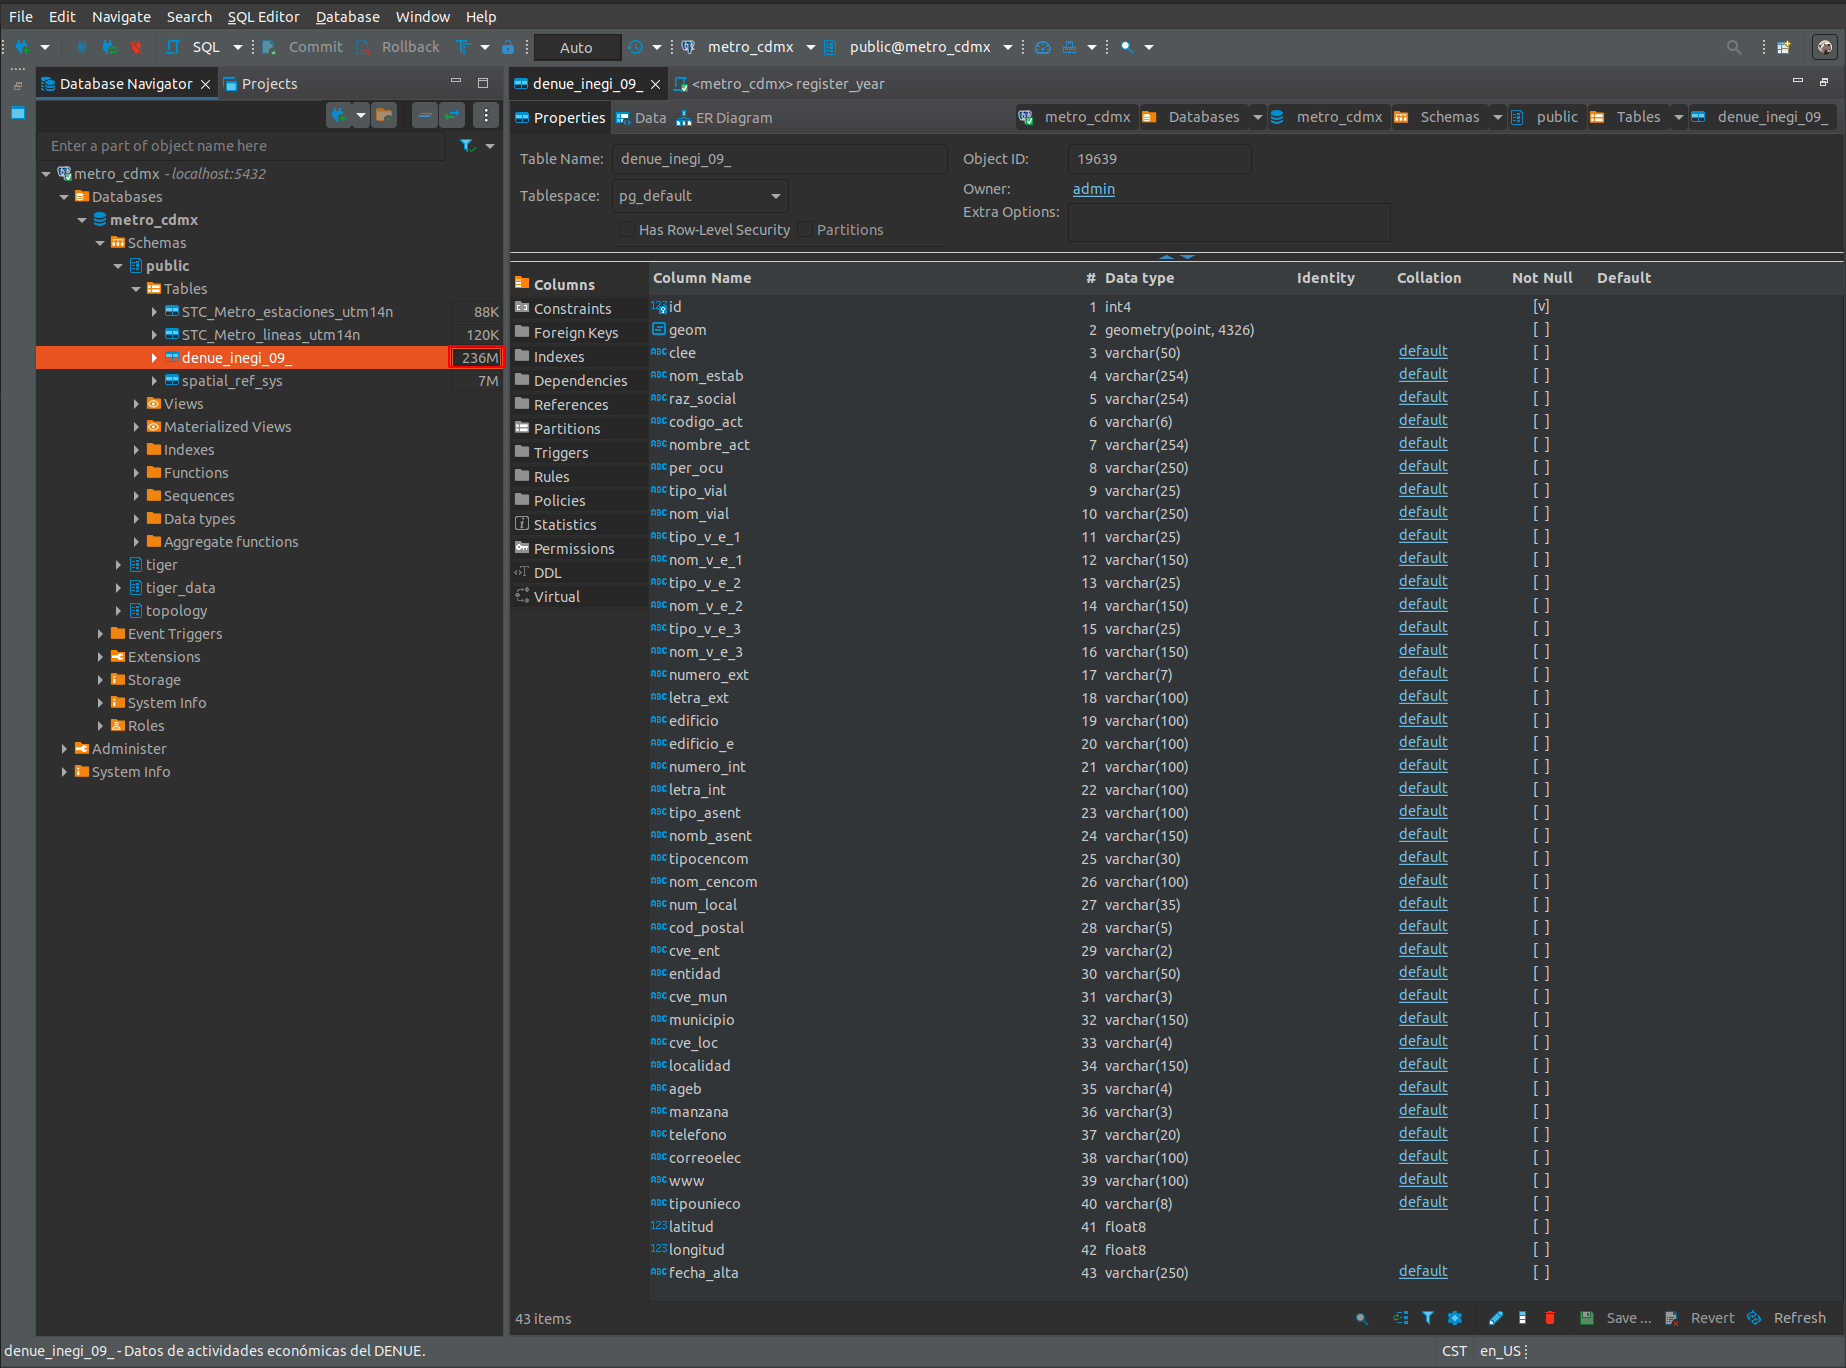
\includegraphics[width=18cm]{figures/bd_original.png}
    \caption{Base de datos antes de la creación de catálogos. Podemos observar
    el espacio ocupado de 236 MB}
    \centering
\end{figure}
\end{landscape}

\begin{figure}[t]
    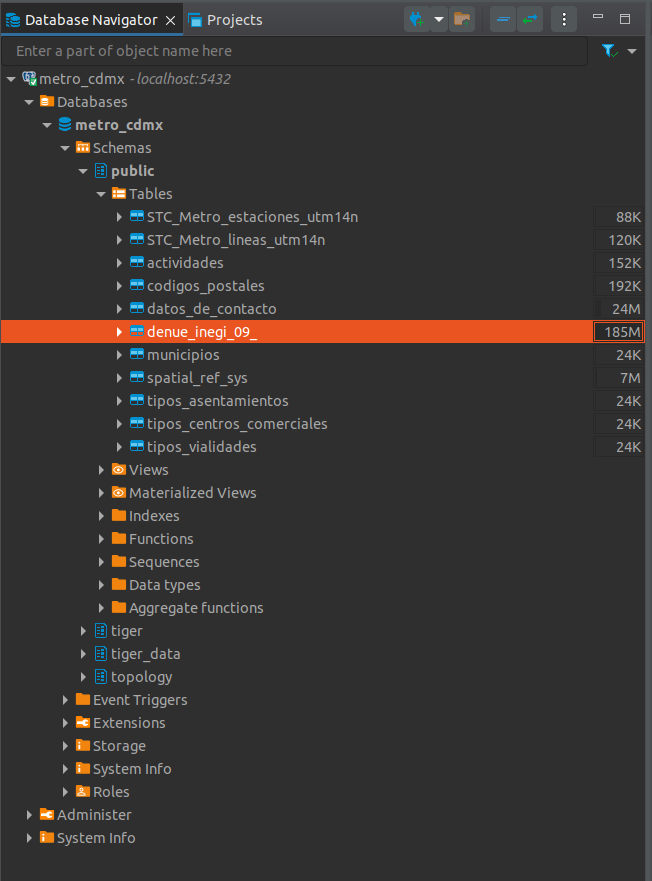
\includegraphics[width=13cm]{figures/bd_actualizada.png}
    \caption{Base de datos después de la creación de catálogos. Podemos observar
    el espacio ocupado por los catálogos, así como el espacio ocupado por la
    base de datos al final de la actualización.}
    \centering
\end{figure}

\end{document}